\subsection{Quest\~{a}o de Pesquisa 1}
\emph{Quais as áreas de SOC são mais frequentemente pesquisadas no contexto de qualidade de serviços?}

%A QP2 tem como objetivo trazer uma perspectiva do cen\'{a}rio das pesquisas em Computa\c{c}\~{a}o Orientada a Servi\c{c}o com foco em QoS atualmente. Para responder a essa pergunta, precisamos primeiramente definir quais s\~{a}o as \'{a}reas que melhor caracterizam as diversas contribui\c{c}\~{o}es de pesquisa em SOC. Da\'{i} ent\~{a}o realizamos a classifica\c{c}\~{a}o.

Para responder a essa pergunta primeiramente identificamos as principais caracter\'{i}sticas de SOC. Encontramos no projeto europeu S-Cube a fundamenta\c{c}\~{a}o mais clara para definir tais caracter\'{i}sticas~\cite{SCube-FINALREPORT} e, portanto, o adotamos como refer\^{e}ncia para definição da faceta da contribui\c{c}\~{a}o. Visando atender ao foco desse estudo, no entanto, adaptamos a estrutura definida no projeto S-Cube. A estrutura proposta foi validada a medida em as publicações puderam ser mapeadas em no mínimo um desses atributos sem maiores dificuldades.

%e obtivemos as seguintes caracter\'{i}sticas: Ciclo de Vida, Composi\c{c}\~{a}o, Coordena\c{c}\~{a}o \& Comunica\c{c}\~{a}o, Descoberta \& Sele\c{c}\~{a}o, Modelos de QoS, Monitoramento \& Adapta\c{c}\~{a}o. 

A Figura~\ref{fig:bubbleplot-QoSSOC} apresenta o diagrama ilustrando a distribui\c{c}\~{a}o dos artigos no eixo horizontal de SOC, a faceta da contribui\c{c}\~{a}o. Assim como os resultados observados nas outras facetas, vale ressaltar que os atributos mapeados não são mutualmente excludentes, visto que representam partes de SOC. Por exemplo, o artigo~\cite{DBLP:conf/dsn/ZhengL09} lida com os composi\c{c}\~{a}o, modelos de QoS \& linguagens assim como monitoramento \& adapta\c{c}\~{a}o. Existe dentre eles alguma sobreposição, notavelmente entre composição \& coordenação. No entanto, notou-se que o termo coordenação tem um significado mais amplo que a própria coordenação de serviços e também envolve aspectos da comunicação entre provedores e consumidores de serviços em geral, independente de composição de serviços. Dessa forma adotamos, em conjunção a coordenação, o termo comunicação.

\begin{figure}[htb]
\centering
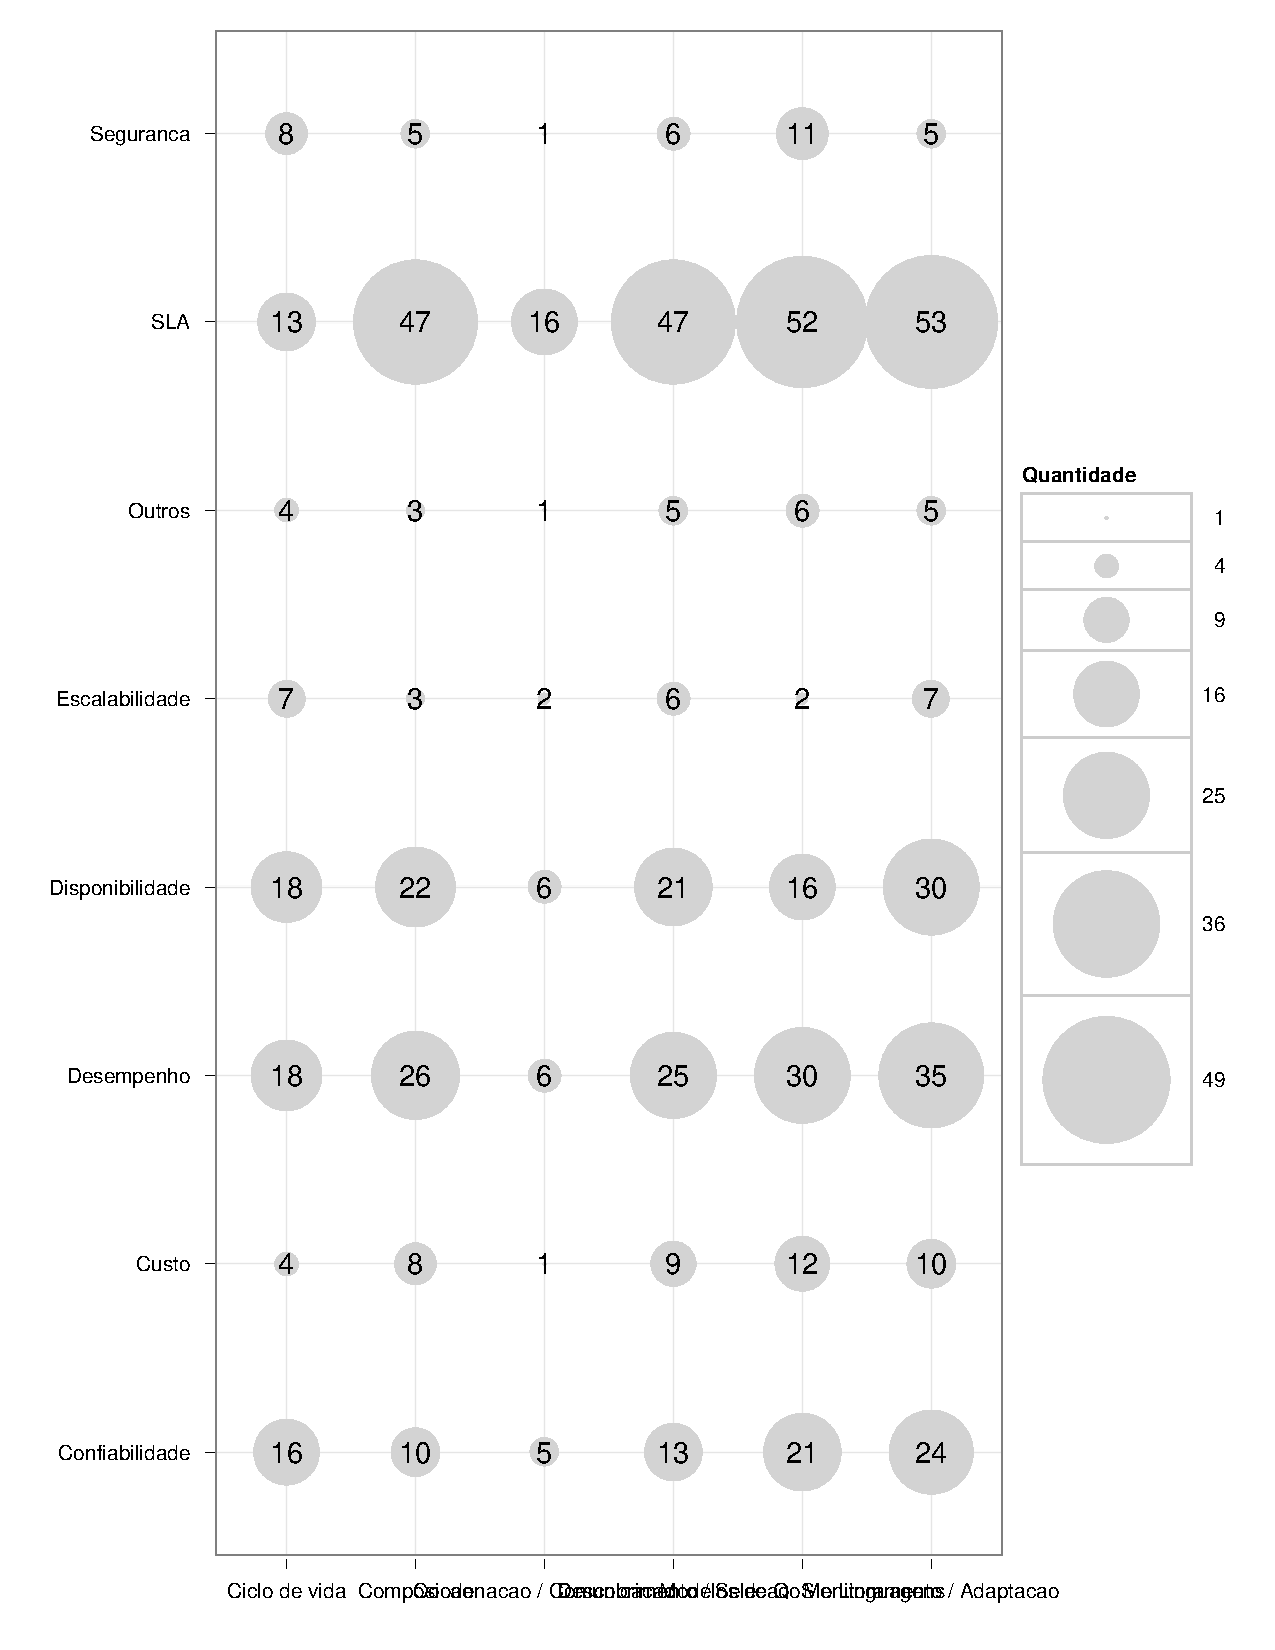
\includegraphics[scale=0.55]{imagens/contribuicaoContexto.pdf}
\caption{\emph{Bubble plot} com a distribui\c{c}\~{a}o ap\'{o}s a realiza\c{c}\~{a}o do primeiro  estudo}
\label{fig:bubbleplot-QoSSOC}
\end{figure}

O resultado desse mapeamento mostra que a maior parte dos trabalhos publicados lida com monitoramento e adapta\c{c}\~{a}o (\MonitoramentoAdaptacao), seguida de modelos de QoS \& linguagens (\ModelosdeQoSeLinguagens), descoberta \& sele\c{c}\~{a}o (\DescobrimentoSelecao),  composi\c{c}\~{a}o (\Composicao), ciclo de vida (\Ciclodevida) e finalmente coordenação com \CoodenacaoComunicacao.

Esses resultados indicam a relevância do monitoramento e adaptação em sistemas baseados em serviços, sobretudo quando aspectos não funcionais  são dinâmicos e podem sofrer variações não só pertinentes à camada de transporte, mas também devido à concorrência, visto que diferentes clientes podem requisitar os mesmos serviços, sobretudo quando a provisão desses é delegada a terceiros. Este modelo de terceirização de serviços é amplamente utilizado pela computação em nuvens, que prevê a provisão de recursos computacionais em termos de infraestrutura, plataforma ou serviços \cite{10.1109/MIC.2010.147}. Dado que o ambiente SOC possui características próprias e diferenciadas, é natural que novas métricas de QoS tenham sido definidas ou que métricas já utilizadas tenham ganho novos significados, assim como linguagens e especificações que admitam o tratamento e negociação dos requisitos de qualidade. O resultado obtido para o atributo de modelos de QoS e linguagens atesta essa contatação. Nota-se também que a descoberta e seleção de serviços foi bem endereçada nas pesquisas, assim como a composição. No primeiro grupo, é considerado o descobrimento e escolha entre serviços de mesma funcionalidade, porém com diferentes níveis de QoS. O segundo abrange não somente a composição, mas também a escolha da melhor configuração de modo a atender aos níveis globais desejáveis ou necessários de QoS para um conjunto de serviços. \textbf{Em relação a ciclo de vida...} Por fim, notou-se um número reduzido de trabalhos que abordam coordenação \& comunicação. 